%
%  Scott Percic
%
\documentclass[12pt,fullpage]{article}
\usepackage{fullpage}
\usepackage{psfrag}                                          % LaTeX graphics tool
\usepackage{pslatex}                                         % avoids the default cmr font
\usepackage{graphicx}                                        % graphics package 
\usepackage{epsfig}                                          % figures
\usepackage{hyperref}
\usepackage{color}

\begin{document}

\noindent
{\bf Extreme value distribution} (from \color{blue}\url{http://www.math.wm.edu/~leemis/chart/UDR/UDR.html}\color{black})

\noindent
The shorthand $X \sim {\rm extreme \ value}(\alpha,\beta)$ is used to indicate that the
random variable $X$ has the extreme value distribution with positive scale parameter $\alpha$ and positive shape parameter $\beta$.
An extreme value random variable $X$ with parameters $\alpha$ and $\beta$ has probability density function 
$$
f(x) = (\beta/\alpha)e^{\kern 0.08 em x \kern 0.08 em \beta-e^{\kern 0.08 em x \kern 0.04 em \beta}/\alpha} \qquad \qquad -\infty<x<\infty.
$$
The extreme value distribution can be used to model water levels associated with floods and earthquake magnitudes.
The probability density function with three different parameter settings is illustrated below.
{\begin{figure}[h!]
\begin{center}
\psfrag{lab1}{$\alpha \kern -0.08 em = \kern -0.08 em 1,\, \beta \kern -0.08 em = \kern -0.08 em 1$}
\psfrag{lab2}{$\alpha \kern -0.08 em  = \kern -0.08 em  1,\, \beta \kern -0.08 em  = \kern -0.08 em  3$}
\psfrag{lab3}{$\alpha \kern -0.08 em  = \kern -0.08 em  5,\, \beta \kern -0.08 em  = \kern -0.08 em  2$}
\psfrag{labx}{$x$}
\psfrag{labf}{$f(x)$}
\includegraphics[width=3.2in]{ExtremevaluePlot.ps}
\end{center}
\end{figure}}

\noindent
The cumulative distribution function is
$$
F(x) =  1 - {{e}^{-{{{e}^{{\it \beta}\,x}}/{\it \alpha}}}} \qquad \qquad -\infty<x<\infty.
$$
The survivor function on the support of $X$ is
$$
S(x) = P(X \ge x) ={{e}^{-{{{e}^{{\it \beta}\,x}}/{\it \alpha}}}} \qquad \qquad -\infty<x<\infty.
$$
The hazard function on the support of $X$ is
$$
h(x) = \frac{f(x)}{S(x)} = {\it \beta}\,{{ e}^{{\it \beta}\,x}}/{\it \alpha} \qquad \qquad -\infty<x<\infty.
$$
The cumulative hazard function on the support of $X$ is
$$
H(x) = {{e}^{{\it \beta}\,x}}/{\it \alpha} \qquad \qquad -\infty<x<\infty.
$$
The inverse distribution function of $X$ is
$$
F ^ {-1}(u) = \frac{\ln  \left(- \alpha \ln
 \left( 1-u \right) \right)}{\beta}
\qquad \qquad -\infty<x<\infty.
$$
The population mean, variance, skewness, and kurtosis of $X$ do not have closed-form expressions.

\vspace{0.05in}

\newpage
\noindent
{\bf APPL verification:}
The APPL statements
\begin{verbatim}
X := ExtremeValueRV(alpha, beta);
CDF(X);
SF(X)
HF(X);
Mean(X);
Variance(X);
Skewness(X);
Kurtosis(X);
MGF(X);
\end{verbatim}
verify the survivor function, hazard function, and cumulative hazard function, and show that the population mean, variance, skewness, kurtosis, and moment generating function
do not have closed-form expressions.
\end{document}
